\section{Theoretische Grundlagen und Stand der Technik}

\subsection{Stand der Technik in der Objekterkennung}

Die moderne Objekterkennung wird heute maßgeblich von Deep-Learning-Ansätzen, insbesondere \textit{Convolutional Neural Networks} (CNNs), dominiert. Diese haben traditionelle Methoden, die auf handgefertigten Merkmalen wie HOG (\textit{Histogram of Oriented Gradients}) basierten, hinsichtlich Genauigkeit und Flexibilität weitgehend abgelöst. CNNs lernen Merkmale direkt aus den Daten und ermöglichen dadurch robustere und besser generalisierbare Modelle.

Innerhalb der Deep-Learning-basierten Objekterkennung existieren zwei Hauptstrategien:

\begin{enumerate}
    \item \textbf{Two-Stage Detectors:} Zunächst werden potenzielle Regionen (\textit{Region Proposals}) generiert, in denen sich Objekte befinden könnten. Anschließend werden diese Regionen klassifiziert (z.B. Faster R-CNN). Diese Ansätze erreichen oft eine hohe Genauigkeit, sind jedoch tendenziell langsamer.
    \item \textbf{One-Stage Detectors:} Hierbei wird die Objekterkennung als direktes Regressionsproblem formuliert. Bounding-Box-Koordinaten und Klassenwahrscheinlichkeiten werden in einem einzigen Durchlauf vorhergesagt. Bekannte Vertreter sind SSD (\textit{Single Shot MultiBox Detector}) und insbesondere YOLO (\textit{You Only Look Once}), die sich durch hohe Verarbeitungsgeschwindigkeit für Echtzeitanwendungen auszeichnen.
\end{enumerate}

\subsubsection{YOLO als Basis für schnelle Detektion}

YOLO unterteilt das Eingabebild in ein Gitter. Jede Zelle ist für die Erkennung von Objekten zuständig, deren Mittelpunkt in sie fällt. Für jede Zelle werden Begrenzungsrahmen, ein Konfidenzwert und Klassenwahrscheinlichkeiten vorhergesagt. 

Seit der ersten Veröffentlichung wurden zahlreiche Weiterentwicklungen (YOLOv3, v4, v5, \ldots, v8 etc.) vorgestellt, die:
\begin{itemize}
    \item die Architektur verfeinerten,
    \item die Genauigkeit, insbesondere bei kleinen Objekten, verbesserten und
    \item Techniken wie Feature Pyramid Networks zur besseren Merkmalsextraktion integrierten.
\end{itemize}

Die Stärke von YOLO liegt in seiner Geschwindigkeit. Daher eignet es sich besonders für die initiale Detektion von Objekten wie Gesichtern oder Kennzeichen in Videoströmen, wie auch in diesem Projekt genutzt.

\subsubsection{MediaPipe für detaillierte Wahrnehmung auf Endgeräten}

Parallel zur Entwicklung von Detektionsarchitekturen wie YOLO gewinnen Frameworks wie Google's MediaPipe an Bedeutung. MediaPipe bietet optimierte, vortrainierte Modelle und komplette, plattformübergreifende Pipelines für spezifische Wahrnehmungsaufgaben direkt auf Endgeräten (Mobilgeräte, Web). 

Es spezialisiert sich auf die effiziente Extraktion detaillierter Informationen, wie:
\begin{itemize}
    \item hochauflösende Gesichtsgitter (\textit{Face Mesh}),
    \item Hand- oder Körper-Landmarken,
\end{itemize}
und ermöglicht damit Anwendungen wie Gestensteuerung, AR-Effekte oder die Analyse biometrischer Merkmale in Echtzeit.

\subsubsection{Kombination von Ansätzen}

Häufig werden verschiedene Ansätze kombiniert. Ein schneller Detektor wie YOLO kann die grobe Position eines Gesichts bestimmen. Anschließend extrahieren spezialisierte Modelle wie MediaPipe detaillierte Landmarken innerhalb der detektierten Region. Dieser hybride Ansatz vereint Geschwindigkeit und Detailgenauigkeit.

Für die Anforderungen dieses Projekts – schnelle und zuverlässige Erkennung von Kennzeichen und Gesichtern sowie die detaillierte Analyse von Gesichtsmerkmalen – sind sowohl die YOLO-Architektur als auch das MediaPipe-Framework relevante Technologien.

\subsection{Funktionsweise von YOLO}

YOLO (\textit{You Only Look Once}) verfolgt einen effizienten Ansatz für die Objekterkennung, der sich durch seine hohe Geschwindigkeit auszeichnet. Anstatt das Bild in mehreren Schritten zu analysieren, betrachtet YOLO das gesamte Bild nur einmal (daher der Name) und sagt alle Objekte gleichzeitig vorher. Man kann sich das wie ein schnelles „Überfliegen“ des Bildes vorstellen.

\begin{figure}[htbp]
    \centering
    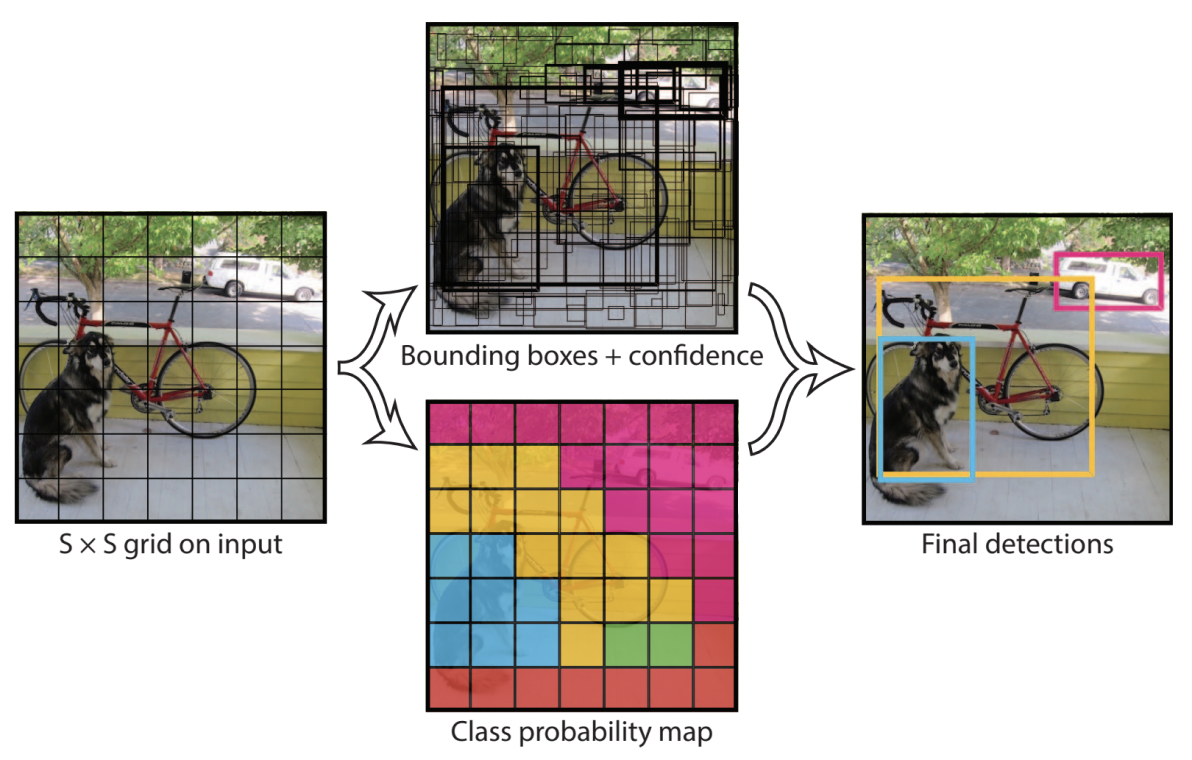
\includegraphics[width=0.8\textwidth]{data/yolo_grid.png}
    \caption{YOLO-Architektur: Das Bild wird in ein Gitter unterteilt, jede Zelle sagt Bounding Boxes und Klassenwahrscheinlichkeiten voraus. Quelle: \cite{yolo_grid}}
    \label{fig:yolo_grid}
\end{figure}

\textbf{Das Gitter (Grid):} \\
Der Kern von YOLO ist die Aufteilung des Eingangsbildes in ein gedachtes Gitter, ähnlich einem Schachbrett (z.B. $13 \times 13$ oder $19 \times 19$ Zellen). Jede dieser Zellen bekommt eine spezielle Aufgabe: Sie ist dafür verantwortlich, Objekte zu erkennen, deren Mittelpunkt genau in diese Zelle fällt.

\textbf{Vorhersagen pro Zelle:} \\
Jede Zelle im Gitter macht mithilfe eines neuronalen Netzes Vorhersagen über mögliche Objekte:
\begin{itemize}
    \item \textbf{Bounding Boxes:} Die Zelle schlägt eine oder mehrere „Boxen“ (Rechtecke) vor, die ein Objekt umschließen könnten. Für jede Box werden Position (x-, y-Koordinaten des Mittelpunkts), Größe (Breite $w$, Höhe $h$) und ein Konfidenzwert vorhergesagt. Dieser Konfidenzwert gibt an, wie sicher sich das Modell ist, dass sich überhaupt ein Objekt in der Box befindet und wie gut die Box passt.
    \item \textbf{Klassenwahrscheinlichkeiten:} Zusätzlich sagt die Zelle voraus, zu welcher Klasse (z.B. „Auto“, „Person“, „Kennzeichen“) ein erkanntes Objekt am wahrscheinlichsten gehört.
\end{itemize}

\textbf{Architektur und Entwicklung:} \\
Das Herzstück ist ein einzelnes Convolutional Neural Network (CNN), das diese Vorhersagen für alle Zellen gleichzeitig generiert. Frühe Versionen nutzten Architekturen wie Darknet. Spätere Versionen (YOLOv3 bis YOLOv8) wurden deutlich komplexer und leistungsfähiger, indem sie z.B. Merkmale aus verschiedenen Ebenen des Netzwerks kombinieren (Feature Pyramid Networks, FPN), um sowohl kleine als auch große Objekte besser zu erkennen. Auch wurden \textit{Anchor Boxes} eingeführt – vordefinierte Box-Formen, die dem Netzwerk helfen, Objekte mit typischen Seitenverhältnissen schneller und genauer zu finden.

\textbf{Aufräumen der Ergebnisse (Non-Max Suppression, NMS):} \\
Da oft mehrere Zellen oder Boxen dasselbe Objekt erkennen, liefert YOLO zunächst viele überlappende Boxen. Um nur die relevanteste Box pro Objekt zu behalten, wird ein „Aufräumschritt“ namens Non-Max Suppression (NMS) durchgeführt. Dabei werden Boxen mit geringer Konfidenz entfernt und von den verbleibenden, überlappenden Boxen wird nur die mit der höchsten Konfidenz behalten, während die anderen verworfen werden.

\textbf{Versionen:} \\
YOLO wird ständig weiterentwickelt. In diesem Projekt kam hauptsächlich YOLOv8 zum Einsatz. Diese Version stellt einen aktuellen Stand der Technik dar und bietet eine gute Balance aus Erkennungsgenauigkeit und hoher Geschwindigkeit, was für die Analyse von Videoströmen vorteilhaft ist. Sie profitiert von den Architekturoptimierungen und Trainingstechniken früherer Versionen und ist oft einfacher zu verwenden. Die Entwicklung schreitet kontinuierlich voran, wie neuere, von Ultralytics dokumentierte Varianten wie YOLOv11 zeigen, was die Dynamik in diesem Bereich unterstreicht.

\subsection{OCR für Texterkennung}

Optical Character Recognition (OCR) bezeichnet den Prozess der Umwandlung von Bildern, die getippten, gedruckten oder handgeschriebenen Text enthalten, in maschinenlesbaren Text. Im Kontext dieses Projekts ist OCR die Schlüsseltechnologie zur Extraktion der Zeichenfolgen aus detektierten Fahrzeugkennzeichen.

\subsubsection{Typische OCR-Pipeline}
Ein OCR-System durchläuft typischerweise mehrere Stufen:

\begin{enumerate}
    \item \textbf{Vorverarbeitung (Preprocessing):} Verbesserung der Bildqualität zur Optimierung der Erkennung. Dies kann Schritte wie Binarisierung (Umwandlung in Schwarz-Weiß), Rauschunterdrückung, Schräglagenkorrektur (Deskewing) und Kontrastanpassung umfassen [Quelle benötigt].

    \item \textbf{Layout-Analyse (oder Segmentierung):} Identifizierung von Textbereichen und deren Struktur. Bei strukturierten Dokumenten wie Kennzeichen kann dies die Segmentierung einzelner Zeichen oder Zeichengruppen umfassen. Bei allgemeineren Texten geht es darum, Absätze, Spalten und Zeilen zu erkennen.

    \item \textbf{Zeichenerkennung (Character Recognition):} Dies ist der Kernschritt, bei dem die segmentierten Zeichen oder Wörter klassifiziert werden. Traditionelle Methoden nutzten Merkmalsextraktion (z.B. topologische Merkmale, Momente) und Klassifikatoren (z.B. SVMs, k-NN). Moderne Ansätze verwenden überwiegend tiefe neuronale Netze, insbesondere CNNs und Recurrent Neural Networks (RNNs), oft in Kombination (CRNN - Convolutional Recurrent Neural Network) [Quelle benötigt - CRNN Paper]. RNNs, speziell LSTMs (Long Short-Term Memory), sind gut geeignet, um sequentielle Informationen in Wörtern oder Zeichenketten zu verarbeiten. Attention-Mechanismen können zusätzlich helfen, relevante Bildbereiche für jedes Zeichen zu fokussieren [Quelle benötigt].

    \item \textbf{Nachverarbeitung (Postprocessing):} Korrektur von Erkennungsfehlern unter Verwendung von Sprachmodellen, Wörterbüchern oder kontextuellen Informationen. Bei Kennzeichen kann dies die Überprüfung auf gültige Formate oder die Nutzung von Prüfsummen (falls vorhanden) beinhalten.
\end{enumerate}

\subsubsection{Methoden und Werkzeuge}
Es existieren verschiedene OCR-Engines und Bibliotheken. Eine der bekanntesten Open-Source-Lösungen ist Tesseract OCR, ursprünglich von HP entwickelt und nun von Google weitergeführt. Tesseract verwendet seit Version 4 LSTM-basierte neuronale Netze und bietet eine gute Erkennungsleistung für viele Sprachen und Schriftarten [Quelle: Tesseract Dokumentation/GitHub]. Daneben gibt es kommerzielle Lösungen und spezialisierte Bibliotheken, die oft für spezifische Anwendungsfälle wie die Kennzeichenerkennung optimiert sind.

\subsubsection{Anwendung bei der Kennzeichenerkennung (ANPR/LPR)}
Automatic Number Plate Recognition (ANPR) oder License Plate Recognition (LPR) ist ein spezialisierter Anwendungsfall von OCR. Die typische Pipeline sieht oft wie folgt aus:

\begin{enumerate}
    \item \textbf{Kennzeichen-Detektion:} Zunächst wird der Bereich des Kennzeichens im Bild lokalisiert. Hierfür eignen sich Objekterkennungsmodelle wie YOLO (siehe Abschnitt 2.2) hervorragend, die darauf trainiert werden, Kennzeichen als Objektklasse zu erkennen [Quelle benötigt].

    \item \textbf{Zeichensegmentierung:} Innerhalb des detektierten Kennzeichenbereichs werden die einzelnen Zeichen isoliert. Dies kann durch traditionelle Bildverarbeitungsalgorithmen (z.B. Konturanalyse, Projektionsprofile) oder durch spezialisierte neuronale Netze erfolgen.

    \item \textbf{Zeichenerkennung:} Jedes segmentierte Zeichen wird durch ein OCR-Modul klassifiziert.
\end{enumerate}

Alternativ können End-to-End-Ansätze verwendet werden, die Detektion und Erkennung in einem einzigen Netzwerk kombinieren oder direkt die gesamte Zeichenkette ohne explizite Segmentierung erkennen [Quelle benötigt].

\subsubsection{Herausforderungen}
Die OCR von Kennzeichen unterliegt spezifischen Herausforderungen wie:
\begin{itemize}
    \item variierenden Lichtverhältnissen (Tag/Nacht, Schatten, Blendung),
    \item unterschiedlichen Kameraperspektiven und -abständen,
    \item Verschmutzung oder Beschädigung der Kennzeichen,
    \item verschiedenen Kennzeichenlayouts und Schriftarten (je nach Land/Region),
    \item Bewegungsunschärfe [Quelle benötigt]
\end{itemize}

Die Robustheit des OCR-Systems gegenüber diesen Faktoren ist entscheidend für die praktische Anwendbarkeit.

\subsection{Gesichtserkennung mit neuronalen Netzen}

Die Gesichtserkennung ist ein Spezialfall der Objekterkennung und der biometrischen Identifikation, die in den letzten Jahren durch den Einsatz neuronaler Netze erhebliche Fortschritte erzielt hat. Sie umfasst typischerweise mehrere Schritte: Gesichtsdetektion, Vorverarbeitung, Merkmalsextraktion und Vergleich oder Klassifikation.

\subsubsection{Technologien im Detail}

\paragraph{Gesichtsdetektion:} 
Wie in Abschnitt 2.1 und 2.2 beschrieben, können Modelle wie YOLO hierfür eingesetzt werden. Alternativ nutzen viele Frameworks dedizierte, oft schnellere Detektoren (z.B. basierend auf SSD oder spezialisierten Architekturen).

\paragraph{Landmarken-Detektion:} 
Frameworks wie Google's MediaPipe bieten spezialisierte Modelle zur Detektion von hunderten von Gesichtslandmarken in Echtzeit (z.B. das Face Mesh mit 468 3D-Landmarken). Diese detaillierten Landmarken sind nicht nur für die Gesichtsausrichtung nützlich, sondern ermöglichen auch die Analyse von Mimik, Augenbewegungen (wie im Projektkontext für Eye Tracking relevant), Kopfbewegungen und die Extraktion geometrischer Merkmale, die potenziell für biometrische Erkennungsansätze genutzt werden können. Die Landmarken selbst können als Merkmalsvektor dienen, obwohl für die reine Identifikation meist Embeddings aus tieferen CNNs verwendet werden.

\paragraph{Embedding-Generierung:} 
Bibliotheken wie face\_recognition (die auf dlib basiert) kapseln oft den Prozess der Detektion, Landmarken-Findung und Embedding-Generierung mithilfe vortrainierter Modelle (z.B. ResNet-basiert). Sie liefern direkt die 128-dimensionalen Embeddings, die dann für den Vergleich genutzt werden können. Diese Bibliotheken vereinfachen die Implementierung von Standard-Gesichtserkennungspipelines.

\subsubsection{MediaPipe Framework für Wahrnehmungsaufgaben}

MediaPipe ist ein Open-Source-Framework von Google, das die Entwicklung komplexer Computer-Vision-Anwendungen erleichtert. Es ermöglicht die Erstellung effizienter, plattformübergreifender Machine-Learning-Pipelines für die Verarbeitung von Video-, Bild- und Audiodaten in Echtzeit. Dank seiner modularen Architektur und der Nutzung vorgefertigter Komponenten, sogenannter ``Calculators'', können Entwickler schnell Prototypen erstellen und diese zu ausgereiften Anwendungen weiterentwickeln.

\paragraph{Graphbasierte Architektur}
Ein zentrales Merkmal von MediaPipe ist seine graphbasierte Architektur. Datenflüsse werden in sogenannten ``Graphs'' definiert, wobei jeder Knotenpunkt (``Node'' oder ``Calculator'') spezifische Aufgaben übernimmt (z.B. Bilddekodierung, Inferenz mit einem ML-Modell, Landmarken-Rendering). Diese Struktur ermöglicht eine flexible und effiziente Verarbeitung von Datenströmen, was besonders für Anwendungen mit hohen Echtzeitanforderungen von Vorteil ist. Die Graphen können komplexe Abhängigkeiten und parallele Verarbeitungspfade abbilden.

\paragraph{Vortrainierte Lösungen}
MediaPipe bietet eine Vielzahl vortrainierter Lösungen (``Solutions'') für gängige Wahrnehmungsaufgaben, darunter:

\begin{itemize}
    \item \textbf{Face Detection:} Schnelle Detektion von Gesichtern.
    \item \textbf{Face Mesh:} Detaillierte Erkennung von 468 3D-Gesichtslandmarken.
    \item \textbf{Iris Tracking:} Präzise Lokalisierung der Iris.
    \item \textbf{Hands:} Erkennung von Handposen und -landmarken.
    \item \textbf{Pose:} Erkennung von Körperposen und -landmarken.
    \item \textbf{Object Detection:} Allgemeine Objekterkennung.
    \item Weitere Lösungen für Aufgaben wie Segmentierung, Haar-Segmentierung etc.
\end{itemize}

Diese Lösungen sind für den Einsatz auf verschiedenen Plattformen (Android, iOS, Web, Desktop) optimiert und können sowohl auf leistungsstarken Servern als auch auf mobilen Geräten oft in Echtzeit betrieben werden. Sie kapseln die Komplexität der zugrundeliegenden Modelle und Graphen und bieten einfache APIs für Entwickler.

\paragraph{Einsatz im Projektkontext}
Im Kontext dieses Projekts wird MediaPipe insbesondere für die detaillierte Analyse von Gesichtsmerkmalen eingesetzt, wie z.B. die Extraktion von Landmarken für die biometrische Erkennung oder das Eye Tracking. Dies ermöglicht eine präzise und effiziente Erfassung relevanter Merkmale, was beispielsweise bei Zutrittskontrollsystemen oder Müdigkeitserkennung von großer Bedeutung ist.

\subsubsection{Vergleich von Latenz und Interferenz (YOLO vs. MediaPipe)}
Bei der Betrachtung von Latenz und Störanfälligkeit (Interferenz) zeigen YOLO und MediaPipe unterschiedliche Charakteristika, die von der spezifischen Aufgabe und Implementierung abhängen:

\paragraph{Latenz:}
\begin{itemize}
    \item \textbf{YOLO:} Als One-Stage Detector ist YOLO für die initiale Objektdetektion im gesamten Bild optimiert und erreicht hierbei oft sehr geringe Latenzen, insbesondere auf geeigneter Hardware (GPUs). Die Latenz skaliert mit der Modellgröße (z.B. YOLOv8n vs. YOLOv8x) und der Eingabeauflösung.
    
    \item \textbf{MediaPipe:} Die Latenz von MediaPipe-Pipelines hängt stark von der spezifischen Aufgabe und dem zugrundeliegenden Graphen ab. Lösungen wie Face Mesh sind für Echtzeit-Performance auf mobilen Geräten optimiert und weisen oft geringe Latenzen auf, insbesondere wenn sie auf einer bereits detektierten Region of Interest (ROI) operieren. Wird jedoch eine Pipeline verwendet, die intern ebenfalls eine Detektion durchführt (z.B. die allgemeine Face Detection Solution), addieren sich die Latenzen der einzelnen Komponenten. Im kombinierten Ansatz (YOLO zur Detektion, MediaPipe zur Landmarken-Extraktion in der ROI) ist die Gesamtlatenz die Summe beider Schritte.
\end{itemize}

\paragraph{Interferenz / Robustheit:}
\begin{itemize}
    \item \textbf{YOLO:} Die Robustheit gegenüber Störungen (z.B. wechselnde Lichtverhältnisse, teilweise Verdeckung, ungewöhnliche Posen) hängt stark vom Trainingsdatensatz und der Modellvariante ab. Größere Modelle sind oft robuster, benötigen aber mehr Rechenleistung. YOLO kann Schwierigkeiten bei sehr kleinen oder dicht gedrängten Objekten haben, obwohl spätere Versionen hier Verbesserungen zeigen.
    
    \item \textbf{MediaPipe:} Die vortrainierten MediaPipe-Lösungen sind in der Regel auf große und diverse Datensätze trainiert und zeigen oft eine gute Robustheit gegenüber Variationen in Beleuchtung und Pose für ihre spezifische Aufgabe (z.B. Face Mesh). Da sie oft auf spezifische Merkmale fokussieren (z.B. Landmarken), können sie bei starker Verdeckung oder untypischen Erscheinungsbildern jedoch ebenfalls an Grenzen stoßen. Die Performance kann auch durch die Qualität der initialen Detektion beeinflusst werden, falls die Pipeline auf einer ROI arbeitet.
\end{itemize}

\subsubsection{Herausforderungen}
Trotz großer Fortschritte bleiben Herausforderungen bestehen:

\begin{itemize}
    \item \textbf{Pose Variation:} Starke Abweichungen von der frontalen Ansicht.
    
    \item \textbf{Illumination:} Ungleichmäßige oder extreme Beleuchtung (Schatten, Gegenlicht).
    
    \item \textbf{Occlusion:} Teile des Gesichts sind verdeckt (Maske, Sonnenbrille, Haare).
    
    \item \textbf{Expression:} Starke mimische Veränderungen.
    
    \item \textbf{Aging:} Veränderungen des Gesichts über die Zeit.
    
    \item \textbf{Resolution / Blurring:} Geringe Bildqualität oder Bewegungsunschärfe.
    
    \item \textbf{Look-alikes:} Hohe Ähnlichkeit zwischen verschiedenen Personen.
    
    \item \textbf{Presentation Attacks (Spoofing):} Versuche, das System mit Fotos, Videos oder Masken zu täuschen (relevant für Kapitel 3.3).
\end{itemize}

Die Robustheit gegenüber diesen Faktoren und die Sicherheit gegen Angriffe sind zentrale Forschungs- und Entwicklungsbereiche in der Gesichtserkennung.

Zusammenfassend lässt sich sagen, dass YOLO oft Vorteile bei der schnellen Initialdetektion im Gesamtbild hat, während MediaPipe seine Stärken in der effizienten und robusten Extraktion spezifischer Merkmale (wie Landmarken) auf Endgeräten ausspielt. Die Wahl oder Kombination hängt von den spezifischen Anforderungen an Geschwindigkeit, Genauigkeit und Robustheit der Anwendung ab.
